%--------------------------------------------------------------------------------------------------------------------------
%                                                   INTRODUCTION
%--------------------------------------------------------------------------------------------------------------------------
The objective of this proposal is to standardize the usage of common data structures within the context of the C language. The existence of a common standard interface for lists, hash tables, flexible arrays, and other containers has several advantages:
\begin{itemize}
\item
User code remains portable across different projects. In C, we all use the FILE abstraction, for instance. This abstraction allows software to be 
compatible across a large spectrum of machines and operating systems. Imagine what would happen if each project had to develop a file stream
abstraction again and again. This is the case when using lists, for instance. Today, we have in all significant projects written in C a list
module, and probably other ones like hash tables, etc. 

\item Avoid duplication of effort. Most of the list or hash tables modules can't be debugged completely and are the source of never ending problems.
\item Lack of standards makes the merging of two projects very difficult since in most cases the interfaces and data structures are slightly
different. This leads to a complete rewrite of one of the modules, or to "adapter" software that will translate from one list implementation
to the other, adding yet another layer of complexity to the merged project.
\item The language becomes more expressive since it becomes possible to reason within a high level environment. The lack of operations for
handling advanced data structures conditions programmers to use low level solutions like making an array with a fixed maximum size instead of a
list even if the programmer would agree that a list would be a more adequate solution to the problem. Confronted to the alternative of
developing yet another list module or opting for a low level solution many time constrained programmers will opt for the second solution.
\item
The portable specifications provide a common framework for library writers and compiler/system designers to build compatible yet strongly specialized implementations.
\item
The language becomes easier to analyze mathematically.
In their very interesting paper "Precise reasoning for programs using containers", Dillig, Dillig and Aiken
\footnote{"Precise Reasoning for programs using containers" Isil Dillig, Thomas Dillig, and Alex Aitken, available on line at
http://www.stanford.edu/\string~isil/popl2011.pdf or at POPL 2011 Proceedings of the 38th annual ACM SIGPLAN-SIGACT symposium on Principles of programming languages
ACM New York, NY, USA ©2011 } enumerate three main points that make program analysis easier using containers:
\begin{enumerate}
\item Understanding the contents of a container doesn't require understanding the container's implementation
\item Verifying container implementations requires different techniques and degrees of automation than verifying their clients. Hence, separating
these two tasks allows us to choose the verification techniques best suited for each purpose.
\item There are orders of magnitude more clients of a container than there are container implementations. This fact makes it possible to annotate
a handful of library interfaces in order to analyze many programs using these containers.
\end{enumerate}
\item It is possible to abstract from the nature of any container (using the \texttt{iterator} construct) what allows a series of algorithms to
be written without having to bind them to a precise data structure. Containers present a uniform interface to the rest of the program.
\end{itemize}
\par
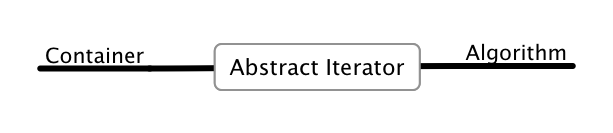
\includegraphics[scale=0.63]{AbstractIterator.png}
\par
The big innovation of C in the eighties was its standard library, that made input/output portable across machines and implementations. The container library would replicate again that idea, at a higher level.

The specifications presented here are completely scoped by the C99 specifications, and can be implemented even in compilers that do not implement C99 and remained within the C94 context. No language extensions are needed nor any are proposed.


The interfaces proposed try to present complete packages, i.e. interfaces with all the necessary functions to allow the widest usage: Serialization, searching, and many other functionalities are included in the proposed standard to allow for maximum code portability. It can be argued that this makes  for "fat" containers, but if you read carefully you will notice that many things can be left out in systems that run in low memory or with feeble computing power.

This documentation is composed of several parts:
\begin{enumerate}
\item An introductory part where the general lines of the library are explained.
\item A specifications part where each function of the library is fully specified. This is the proposal for the next C standard.
\item An "examples" part that shows the uses of the library and allows you to have a better idea of how the usage of the library looks like.
\item An implementation part where the code of the sample implementation is discussed. This is designed as a guide for implementors to give them a basis to start with.
\end{enumerate}
%
%---------------------------------------------------------------------------Design Goals
%
\section{Design goals}
\subsection{Error analysis}
It has been a  tradition in C to place raw performance as the most important quality of specifications. To follow this sacred cow, C specifications
ignored any error analysis arguing that any specification of failure modes would damage "performance". No matter that raw machine performance
increased by several orders of magnitude, the cost of  a check for NULL was always "too expensive" to afford.

This kind of mental framework was described by one of the people in the discussion group "comp.lang.c++" as follows:\footnote{We were discussing 
the specifications of the \texttt{mismatch} function of the C++ STL and why any error analysis is absent. The C++ STL prescribes a bounded 
region for the first container, but just a starting point for the second one. If the second is shorter than the specified range of the first
 \textsl{undefined behavior} ensues and anything can happen. In many cases this "anything" is different each time the same error occurs. In our
specific case \texttt{mismatch} would read from memory that doesn't belong to the container it started with. Depending on the contents of
that memory a crash could happen, or worst, a wrong result returned to the calling software, etc.}
\begin{quotation}
 In C++, the program is responsible for ensuring that \textbf{all} parameters to
 the standard library functions are valid, not only the third parameter of
 \texttt{std::mismatch()}. For example, also the first range for \texttt{std:mismatch()}
 must be valid, one may not pass a start iterator from one container and
 end iterator from another, for example. However, STL does not guarantee
 any protection against such errors, this is just UB.
\end{quotation}
These specifications try to break away from that frame of thought. Each function specifies a minimal subset of failure modes as a consequence of its 
error analysis. This allows user code to:
\begin{itemize}
\item Detect and handle errors better. Error detection is simple: Almost all functions return a negative
error code when they detect an error condition. Error detection can always test for the result
of any API with:
\begin{verbatim}
if (SomeCclApi(arg1,arg2) < 0) {
    // error handling here
}
\end{verbatim}

Some functions like the \verb,Create, function return a pointer. In those cases an error provokes a NULL 
pointer result. The error checking in those cases should be:
\begin{verbatim}
if ((r=SomeCclApi(arg1,arg2)) == NULL) {
    // error handling here
}
\end{verbatim}
\item Ensure that errors will always have the \textbf{same} consequences. One of the worst consequences of undefined behavior is that the same error can 
have completely different consequences depending on apparently random factors like previous contents of memory or previous allocation pattern.
\end{itemize}

At the same time, the mandatory error checking consists mainly of checks that can be implemented with a few integer comparisons. For instance a check 
for zero is a single instruction in most processors. If implemented correctly the conditional jump after the comparison with zero is not taken in the 
normal case and correctly predicted by the processor. This means that the pipeline is not disturbed and the cost for the whole operation is much less than a cycle.

Why is error analysis an essential part of any program specifications?

Because \textbf{mistakes are a fact of life}. Good programmers are good most of the time only. Even very good programmers \textsl{do make mistakes\footnote{Donald Knuth, the author of the TeX typesetting program can be without doubt be qualified as a good programmer (and an excellent computer scientist). But he, like anybody else, is not without flaws. See: 
www.tug.org/texmf-dist/doc/generic/knuth/errata/errorlog.pdf. There are hundreds of entries in that log.}.} Software
must be prepared to cope with this fact in an orderly fashion because if failure modes are not specified they have catastrophic consequences and lead
to brittle software that crashes randomly.

Note that error \textsl{analysis} is not error \textsl{handling}. Error handling is taking an action after an error, a task only the application can do.
What the library can do is to establish a framework where a user defined procedure receives enough information about the specific problem at hand.

Error analysis means that for each function and each API:
\begin{itemize}
\item An analysis is performed of what are the consequences of any error in its inputs. Error codes are used to pass detailed error information
to the error procedure.
\item During its execution, an analysis is done of each step that can fail.
\item The outputs of the function are left in a consistent state, errors provoking the undo of the previous steps in most cases, leaving the inputs
as they were before the function was called. This feature allows library functions to be restartable after an error. For instance an out of memory
condition can be corrected by freeing memory and retrying.
\end{itemize}
The library provides hooks for the users that can control each step and provide functions that can do the error handling, for instance logging the
error and jumping to a pre-established recovery point.
\subsection{Full feature set}
Another design goal is to offer to the user a full feature set, complete with serializing, iterators, search, read-only containers and all the features 
needed in most
situations. Other features are planned for later like multi-threading support. The objective here is to avoid incompatible and non portable extensions
because some essential feature is missing.
\subsection{Abstraction}
The library is designed with the possibility of implementing abstraction like serial and associative containers that allow software to treat several 
containers in a way that abstract most of their features, improving code reuse by allowing to implement algorithms for a class of objects. This is
specially true in the iterators feature.

It can be argued that the C language lacks many of the abstractions constructs of other languages like templates, inheritance, and many others.
All that is true, but the objective of this proposal is to show that those constructs are just an aid to developing abstractions, an aid that
is paid in added complexity for the resulting language, and in a limitation of what is feasible within a given framework. Since C has no 
framework, no preferred inheritance model, it is possible to create abstractions that are quite unconstrained: there is no framework precisely.
\subsection{Performance} Even with all the tests, the performance of the library has been maintained at a high level compared to similar libraries
in other languages. The performance should improve if standardized because compiler writers could specialize their optimizations targeting this
code.
\subsection{Compile time checking}
The base implementation of the library uses \verb,void *, everywhere since the library can't know what type
of data the user is storing in it. This means that no compile-time checking can be done on the type of
arguments passed to a library function, what is very error prone.

To mitigate this problem the library offers a "templated" version of each container, where the user must
write a very small parameter file for a templated version that specifies a container for a specific data
type, allowing for compile time checking of arguments and a simpler syntax.

Note that no new language features are needed for this to work since it uses the preprocessor to specialize
a file template of the desired container. Most of the containers are provided in these two forms: a generic
version using void pointers and a templated version that builds a software layer between the generic version and
the specialized version allowing for compile time checking.

To speed up this process specialized versions of the list and vector containers are provided for most of the
basic types of the language: int, doubles, etc.
\subsection{Design choices}
The parameter space for a container library is virtually infinite. There are choices and choices to be made and it would be
impossible to explain them all. There are choices done by default (the other possibilities aren't realized or not even considered)
or choices made semi-consciously ("... it is better not to go in that direction") or done because
other choices done before impose them. And there are choices done with full knowledge of the alternatives,
where a conscious choice is done after exploring several possible solutions.

Here are some examples of design decisions, to show the kind of reasoning that goes into them,
and the priorities schema.
\begin{itemize}
\item Some libraries propose the use of "invasive" containers where the user defines
some fields \textsl{within his/her structure definitions} where the containers
would have a handle to act. For instance the user defines a single field "Next" within
his data structure definition so that the single linked list container can use it
to perform its operations.

The problem with this approach is that all the fields necessary must be fully disclosed
to the user. Any change in those fields provokes a recompilation of \textsl{all} user
codes. There isn't really a full separation between the container data structures
and the user's.

A big design goal is the complete separation of the containers from user's code so that
a new version of the library doesn't need any changes to user code at all, not even
to the binaries. Within the current design the implementor of the library can change
the inner structure of its data structures without affecting at all user's code.

\item Another design decision is to hide or not the container access within macros. Instead
of writing: 
\begin{verbatim}
    iList.Add(myList,&mydata);
    iVector.Add(myVector,&mydata) 
// that would be replaced by
#define CCL_ListAdd(myList,mydata) iList.Add(myList,&mydata)
#define CCL_VectorAdd(myVector,mydata) iVector.Add(myVector,&mydata)
// ... etc
\end{verbatim}

This  has been a very difficult design decision, and one that is not closed yet.
The advantage of this is that the implementor can then make hidden functions that
inline calls, and in general increase the speed of the generated code. 

Another advantage is that the linker
doesn't need to include \textbf{all} members of the list container but only
those that are used into the final executable.

The problem is that this is (in my opinion) \textbf{too} flexible and hides
completely what is happening from the user. Another problem is that even if the
new names are all prefixed (here with \verb,CCL_,) name clashes can occur. The
resulting names are quite long also, even if typing \verb,iList.Add, is also
quite long.

Here the decision is not definitive since at any moment a set of macros can be added
to the library.
\end{itemize}
%-----------------------------------------------------------------------------------------------------------
%                                                       Typographical conventions
%-----------------------------------------------------------------------------------------------------------
\section{How the functions are specified in this document.}
The specifications part of the proposal uses the same building blocks for each of the functions proposed.\par\noindent
\textbf{Name}

\noindent The name of the function. Note that when using this name, the name of the container interface should be always before 
since this name is a field of the interface structure:

\noindent \verb,iList.Add,, \verb,iDictionary.Add,, etc.

\noindent The name is followed by the prototype defined as a function pointer. For the function \verb,Add, of the container \verb,List, we have
\begin{verbatim}
    int (*Add)(List *list,const void *data);
    int (*Add)(TYPEList *list,const TYPE data);
\end{verbatim} 
This means that \verb,Add, is a function pointer in the interface \verb,iList,. It would be used as:
\texttt{iList.Add(list,data)}.
The second line corresponds to the \textsl{template} form of the API. This is explained further down (\S \ref{TwoTypes} page-\pageref{TwoTypes}) and
it is specified only when the signature of the API diverges from the generic one. The \verb,TYPE, marker means that
a type name should appear there: in the example it could be intList, doubleList, CustomerList, etc.

\apidescription The API is described: purpose, inputs and outputs. Note that unmodified arguments are always marked
as \verb,const,.

\apierrors
The minimal set of errors that can appear during the execution of the function is listed. Each implementation 
is free to add implementation specific errors to this list. Note that how the library behaves after an error is 
defined by the current error function in the container (if any), then by the behavior of the error function in the 
\verb,iError, interface.

\returns
The return value of the operation. Normally, negative values are error codes, positive values means success, and zero means non fatal errors, more in the sense of a warning.

\section{Which sections of this document are normative?}
This document presents the C container Library to the C standardization committee. The following sections are normative:
\begin{itemize}
\item Chapter 4: The auxiliary interfaces. The required interfaces are:
\begin{ShorterItemize}
\item The mask interface
\item The memory management interface
\item The error handling interface
\item The iterator interface
\item The observer interface
\end{ShorterItemize}

The heap and pool interfaces are optional.
\item Chapter 5: The containers:
\begin{center}
\begin{longtable}{|p{2.7cm}|p{3cm}|p{2.1cm}|p{6.0cm}|}
\hline
\textbf{Container}&\textbf{Interface}&\textbf{Required?}&\textbf{Short description}\\\hline
BitString&iBitString& \Checkmark &\footnotesize{Sequence of bits}\\
BloomFilter&iBloomFilter&\XSolidBrush &\footnotesize{Statistical container}\\
CircularBuffer&iCircularBuffer& \Checkmark &\footnotesize{Retains the last $n$ items}\\
Deque&iDeque&\Checkmark &\footnotesize{Queue with fast insertions at both ends.}\\
Dictionary&iDictionary&\Checkmark& \footnotesize{Associates a character key to arbitrary data.} \\
Dlist&iDlist&\Checkmark &\footnotesize{Double linked list}\\
HashTable&iHashTable&\XSolidBrush &\footnotesize{Associates a key with data.}\\
List&iList&\Checkmark &\footnotesize{Single linked list.}\\
Queue&iQueue&\Checkmark &\footnotesize{First in, first out container.}\\
PQueue&iPriorityQueue&\Checkmark &\footnotesize{Pull out items by priority.}\\
StreamBuffer&iStreamBuffer&\Checkmark &\footnotesize{Sequence of bytes.}\\
StringList&iStringList&\Checkmark&\footnotesize{List of character strings.}\\
strCollection&istrCollection&\Checkmark &\footnotesize{Array of character strings.}\\
TreeMap&iTreeMap&\Checkmark &\footnotesize{Tree structure associates key with data.}\\
Value array&iValArrayXXX&\Checkmark &\footnotesize{Vector of numbers.\footnote{
The different ValArray containers should
include several basic data types like int, char or long.
Floating point types float and double are required, but not the types long long, long double and all complex types.
The rationale is to avoid excluding C implementations designed for very small processors or environments.}}\\
Vector&iVector&\Checkmark &\footnotesize{General resizable vector}\\
WstrCollection&iWstrCollection&\XSolidBrush&\footnotesize{Array of wide character strings.}\\
\hline
\end{longtable}
\end{center}
\end{itemize}
All text in footnotes, tables or drawings is not normative.

The order of the APIs within each interface is implementation defined. In general no assumptions should 
exist about any specific layout of the interfaces or data structures in the library. In the documentation
the APIs are listed following the alphabetical order.

The code of the sample implementation can be obtained from:

\noindent\verb,http://code.google.com/p/ccl/,

Go to Downloads and there you will find the documentation (this document) and the source code in the form of a \verb,ccl.zip, file.
\index{Download!source} See also the chapter about the sample implementation in this document.

